\begin{center}
    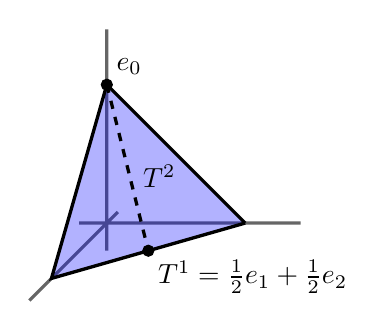
\begin{tikzpicture}[x=1em, y=1em, z=-0.4em, baseline=0.8em]
    \draw[very thick, black!60] 
        (-1,0,0) -- (7,0,0)
        (0,-1,0) -- (0,7,0)
        (0,0,-1) -- (0,0,7);
    \fill[fill=blue, opacity=0.3]
        (5,0,0)--(0,5,0)--(0,0,5)--(5,0,0);
    \draw[very thick, black]
        (5,0,0)--(0,5,0)--(0,0,5)--(5,0,0);
    \draw[dashed, very thick] (0,5,0) -- (2.5,0,2.5);
    \filldraw 
        (0,5,0) circle (2pt) node[anchor=south west] {$e_0$}
        (2,3.5,2.6) node[anchor=north west] {$T^2$}
        (2.5,0,2.5) circle (2pt) node[anchor=north west] {$T^1=\frac{1}{2}e_1+\frac{1}{2}e_2$};
    \end{tikzpicture}$\quad\quad\quad\quad$
    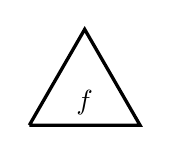
\begin{tikzpicture}[x=4em, y=4em, baseline=0.8em]
    \draw[very thick] (0,0) -- (1,0) -- (0.5, 0.866) -- (0,0);
    \filldraw (0.5, 0.2) node {$f$};
    \end{tikzpicture}$+$
    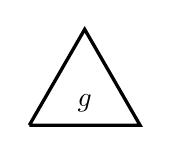
\begin{tikzpicture}[x=4em, y=4em, baseline=0.8em]
    \draw[very thick] (0,0) -- (1,0) -- (0.5, 0.866) -- (0,0);
    \filldraw (0.5, 0.2) node {$g$};
    \end{tikzpicture} $=$
    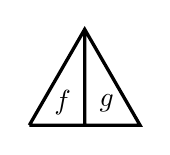
\begin{tikzpicture}[x=4em, y=4em, baseline=0.8em]
    \draw[very thick] (0,0) -- (1,0) -- (0.5, 0.866) -- (0,0)
    (0.5,0)--(0.5, 0.866);
    \filldraw (0.3, 0.2) node {$f$}
    (0.7, 0.2) node {$g$};
    \end{tikzpicture}
\end{center}